\documentclass[aspectratio=169,10pt]{beamer}

% ============================================================
% OmniCast - Joint Project Defense Presentation Slide Deck
% Courses: PRN232 (Back-End) & PRM393 (Mobile Client)
% Academic Semester: Fall 2026 (FA26) - FPT University
% ============================================================

\usepackage{fontspec}
\setmainfont{Arial}
\setsansfont{Arial}
\setmonofont{Consolas}

\usepackage{tikz}
\usetikzlibrary{calc,positioning,arrows.meta,shapes.geometric,fit,backgrounds}
\usepackage{booktabs}
\usepackage{tabularx}
\usepackage{xcolor}
\usepackage{url}
\usepackage{listings}
\usepackage{tcolorbox}
\tcbuselibrary{skins,breakable}

% ---------- OmniCast Cinema Dark Color Scheme ----------
\definecolor{omniDark}{HTML}{0B132B}
\definecolor{omniCard}{HTML}{16203A}
\definecolor{omniDeep}{HTML}{070C1B}
\definecolor{omniCyan}{HTML}{00E5FF}
\definecolor{omniBlue}{HTML}{38BDF8}
\definecolor{omniTeal}{HTML}{14B8A6}
\definecolor{omniPurple}{HTML}{A78BFA}
\definecolor{omniAmber}{HTML}{FBBF24}
\definecolor{omniGreen}{HTML}{34D399}
\definecolor{omniSlate}{HTML}{94A3B8}
\definecolor{omniBorder}{HTML}{2A3756}
\definecolor{omniLight}{HTML}{F8FAFC}

% ---------- Beamer Theme Settings ----------
\setbeamercolor{background canvas}{bg=omniDark}
\setbeamercolor{normal text}{fg=omniLight}
\setbeamercolor{title}{fg=white}
\setbeamercolor{subtitle}{fg=omniCyan}
\setbeamercolor{author}{fg=omniSlate}
\setbeamercolor{date}{fg=omniSlate}
\setbeamercolor{frametitle}{fg=white,bg=omniDark}
\setbeamercolor{structure}{fg=omniCyan}
\setbeamercolor{item}{fg=omniCyan}

\setbeamertemplate{navigation symbols}{}

% ---------- Custom Header & Footer ----------
\setbeamertemplate{headline}{
  \leavevmode
  \begin{tikzpicture}[remember picture, overlay]
    \fill[omniDeep] (current page.north west) rectangle ($(current page.north east) + (0,-10mm)$);
    \draw[omniBorder, line width=0.5pt] ($(current page.north west) + (0,-10mm)$) -- ($(current page.north east) + (0,-10mm)$);
    \node[anchor=west, text=omniCyan, font=\scriptsize\bfseries] at ($(current page.north west) + (8mm,-5mm)$) {OMNICAST};
    \node[anchor=west, text=omniSlate, font=\scriptsize] at ($(current page.north west) + (26mm,-5mm)$) {$\vert$ \ \insertsectionhead};
    \node[anchor=east, text=omniSlate, font=\tiny] at ($(current page.north east) + (-8mm,-5mm)$) {FPT UNIVERSITY $\bullet$ FA26};
  \end{tikzpicture}
  \vspace{8mm}
}

\setbeamertemplate{footline}{
  \leavevmode
  \begin{tikzpicture}[remember picture, overlay]
    \fill[omniDeep] (current page.south west) rectangle ($(current page.south east) + (0,6mm)$);
    \draw[omniBorder, line width=0.5pt] ($(current page.south west) + (0,6mm)$) -- ($(current page.south east) + (0,6mm)$);
    \node[anchor=west, text=omniSlate, font=\tiny] at ($(current page.south west) + (8mm,3mm)$) {OmniCast: Enterprise Media \& Broadcast Intelligence Network};
    \node[anchor=center, text=omniSlate, font=\tiny] at ($(current page.south) + (0,3mm)$) {PRN232 (Back-End) \& PRM393 (Mobile Applications)};
    \node[anchor=east, text=omniCyan, font=\tiny\bfseries] at ($(current page.south east) + (-8mm,3mm)$) {\insertframenumber{} / \inserttotalframenumber{}};
  \end{tikzpicture}
}

\setbeamertemplate{frametitle}{
  \vspace*{2mm}
  \begin{beamercolorbox}[wd=\paperwidth,ht=4ex,dp=1ex,leftskip=8mm]{frametitle}
    {\large\bfseries\insertframetitle}
    \ifx\insertframesubtitle\@empty\else
      \ \ {\footnotesize\color{omniSlate}--- \insertframesubtitle}
    \fi
  \end{beamercolorbox}
}

% ---------- Custom Visual Card Command using Native Beamer Blocks ----------
\setbeamertemplate{blocks}[rounded][shadow=true]

\newcommand{\card}[4]{%
  \begingroup
  \setbeamercolor{block title}{bg=omniDeep,fg=#2}%
  \setbeamercolor{block body}{bg=omniCard,fg=omniLight}%
  \begin{block}{\scriptsize\bfseries #3}%
    \scriptsize #4%
  \end{block}%
  \endgroup
}

% ---------- Title Information ----------
\title{OMNICAST}
\subtitle{Enterprise Media \& Broadcast Intelligence Network}
\author{OmniCast Engineering Team}
\institute{Department of Software Engineering --- FPT University}
\date{Fall Semester 2026 (FA26)}

\begin{document}

% ============================================================
% SLIDE 1: Title Slide (Full Bleed Cinema Dark)
% ============================================================
{
\setbeamertemplate{headline}{}
\setbeamertemplate{footline}{}
\begin{frame}[plain]
  \begin{tikzpicture}[remember picture, overlay]
    \fill[omniDeep] (current page.north west) rectangle (current page.south east);
    \draw[omniCyan!25, line width=0.8pt, dashed] ($(current page.north west) + (10mm,-10mm)$) rectangle ($(current page.south east) + (-10mm,10mm)$);
    \draw[omniBorder, line width=1.2pt] ($(current page.north west) + (12mm,-12mm)$) rectangle ($(current page.south east) + (-12mm,12mm)$);
    \fill[omniCyan] ($(current page.north west) + (12mm,-12mm)$) circle (2.5pt);
    \fill[omniCyan] ($(current page.north east) + (-12mm,-12mm)$) circle (2.5pt);
    \fill[omniCyan] ($(current page.south west) + (12mm,12mm)$) circle (2.5pt);
    \fill[omniCyan] ($(current page.south east) + (-12mm,12mm)$) circle (2.5pt);
  \end{tikzpicture}

  \begin{center}
    \vspace*{-4mm}
    {\scriptsize\bfseries\color{omniSlate}FPT UNIVERSITY $\bullet$ FACULTY OF INFORMATION TECHNOLOGY}\\[2mm]
    {\tiny\color{omniCyan}\bfseries FINAL CAPSTONE DEFENSE \& PROJECT PRESENTATION}\\[4mm]

    {\Huge\bfseries\color{white}OMNI\textcolor{omniCyan}{CAST}}\\[1.5mm]
    {\large\bfseries\color{omniSlate}Enterprise Media \& Broadcast Intelligence Network}\\[3mm]
    
    {\color{omniBorder}\rule{0.65\linewidth}{1pt}}\\[3mm]

    
\begin{tikzpicture}
      \node[draw=omniBlue, fill=omniCard, rounded corners=3pt, line width=0.8pt, inner sep=4pt] (b1) at (-3.2,0) {
        \textbf{\scriptsize\color{white}PART 1: PRN232} \ \textcolor{omniSlate}{\tiny$\vert$} \ \textsf{\scriptsize\color{omniBlue}Back-End Engineering \& Web Portal}
      };
      \node[draw=omniPurple, fill=omniCard, rounded corners=3pt, line width=0.8pt, inner sep=4pt] (b2) at (3.2,0) {
        \textbf{\scriptsize\color{white}PART 2: PRM393} \ \textcolor{omniSlate}{\tiny$\vert$} \ \textsf{\scriptsize\color{omniPurple}Mobile Application (Flutter \& Dart)}
      };
    \end{tikzpicture}
    \vspace{4mm}

    
\begin{tikzpicture}
      \node[text=omniGreen, font=\tiny\bfseries] at (-3.8,0) {$\checkmark$ 142,897 Physical LOC};
      \node[text=omniCyan, font=\tiny\bfseries] at (0,0) {$\checkmark$ 482/482 Tests PASS (100\%)};
      \node[text=omniAmber, font=\tiny\bfseries] at (4.2,0) {$\checkmark$ Live Production on Vercel \& Supabase};
    \end{tikzpicture}
    \vspace{4mm}

    {\scriptsize\color{omniSlate}Author: \textbf{\color{white}OmniCast Engineering Team} $\bullet$ Academic Semester: \textbf{\color{white}Fall 2026 (FA26)}}\\[1mm]
    {\tiny\color{omniSlate}October 28, 2026}
  \end{center}
\end{frame}
}

% ============================================================
% SLIDE 2: Executive Summary & Problem Statement
% ============================================================
\section{Overview}
\begin{frame}{Executive Summary}{The Industry Challenge \& The OmniCast Solution}
  \begin{columns}[t]
    \begin{column}{0.48\textwidth}
      \card{\linewidth}{omniAmber}{THE PROBLEM: BROADCAST COLLISION \& FRAGMENTATION}{
        \begin{itemize}
          \setlength\itemsep{1.5mm}
          \item \textbf{Airtime Collisions:} Overlapping broadcast events cause stream disruptions and schedule inconsistencies.
          \item \textbf{24/7 EPG Dead Air:} Linear TV grids leave empty slots if content runs short, resulting in blank viewer screens.
          \item \textbf{Manual Content Curation:} Broadcasters manually tag, rate, and check compliance across high-volume video catalogs.
          \item \textbf{Rigid Mobile Experiences:} Mobile players freeze without network connection, discarding pending user actions.
        \end{itemize}
      }
    \end{column}

    \begin{column}{0.48\textwidth}
      \card{\linewidth}{omniCyan}{THE OMNICAST SOLUTION: UNIFIED HYBRID ECOSYSTEM}{
        \begin{itemize}
          \setlength\itemsep{1.5mm}
          \item \textbf{Mathematical Collision Engine:} Single SQL interval query prevents airtime overlaps at database transaction level.
          \item \textbf{Seeded 24/7 EPG Auto-Filler:} Fills schedule gaps deterministically with reproducible, channel-specific fallback content.
          \item \textbf{AI Broadcast Curator:} LLM-driven structured metadata curation with Zod schema validation and heuristic fallback.
          \item \textbf{Offline-First Mobile Client:} SQLite caching with pending mutation queue and low-latency WebRTC/HLS streaming.
        \end{itemize}
      }
    \end{column}
  \end{columns}
\end{frame}

% ============================================================
% SLIDE 3: End-to-End System Architecture (The Big Picture)
% ============================================================
\begin{frame}{End-to-End System Architecture}{Dual-Platform Unified Topology}
  \begin{center}
  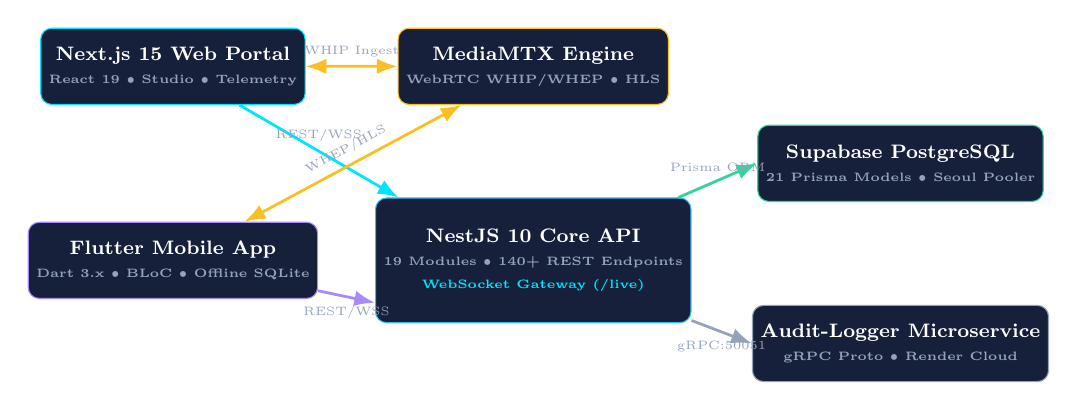
\begin{tikzpicture}[scale=0.88, every node/.style={transform shape, align=center}]
    \node[draw=omniCyan, fill=omniCard, rounded corners=4pt, text=white, font=\footnotesize\bfseries, minimum width=38mm, minimum height=11mm] (web) at (0, 2.2) {Next.js 15 Web Portal\\{\tiny\color{omniSlate}React 19 $\bullet$ Studio $\bullet$ Telemetry}};
    \node[draw=omniPurple, fill=omniCard, rounded corners=4pt, text=white, font=\footnotesize\bfseries, minimum width=38mm, minimum height=11mm] (mob) at (0, -0.6) {Flutter Mobile App\\{\tiny\color{omniSlate}Dart 3.x $\bullet$ BLoC $\bullet$ Offline SQLite}};

    \node[draw=omniAmber, fill=omniCard, rounded corners=4pt, text=white, font=\footnotesize\bfseries, minimum width=32mm, minimum height=11mm] (mtx) at (5.2, 2.2) {MediaMTX Engine\\{\tiny\color{omniSlate}WebRTC WHIP/WHEP $\bullet$ HLS}};

    \node[draw=omniBlue, fill=omniCard, rounded corners=4pt, text=white, font=\footnotesize\bfseries, minimum width=42mm, minimum height=18mm] (api) at (5.2, -0.6) {NestJS 10 Core API\\{\tiny\color{omniSlate}19 Modules $\bullet$ 140+ REST Endpoints}\\{\tiny\color{omniCyan}WebSocket Gateway (/live)}};

    \node[draw=omniGreen, fill=omniCard, rounded corners=4pt, text=white, font=\footnotesize\bfseries, minimum width=35mm, minimum height=11mm] (db) at (10.5, 0.8) {Supabase PostgreSQL\\{\tiny\color{omniSlate}21 Prisma Models $\bullet$ Seoul Pooler}};
    \node[draw=omniSlate, fill=omniCard, rounded corners=4pt, text=white, font=\footnotesize\bfseries, minimum width=35mm, minimum height=11mm] (grpc) at (10.5, -1.8) {Audit-Logger Microservice\\{\tiny\color{omniSlate}gRPC Proto $\bullet$ Render Cloud}};

    \draw[-{Latex}, omniCyan, line width=1pt] (web) -- node[above, font=\tiny, text=omniSlate]{REST/WSS} (api.155);
    \draw[-{Latex}, omniPurple, line width=1pt] (mob) -- node[below, font=\tiny, text=omniSlate]{REST/WSS} (api.195);
    \draw[{Latex}-{Latex}, omniAmber, line width=1pt] (web) -- node[above, font=\tiny, text=omniSlate]{WHIP Ingest} (mtx);
    \draw[{Latex}-{Latex}, omniAmber, line width=1pt] (mob) -- node[above, font=\tiny, text=omniSlate, sloped]{WHEP/HLS} (mtx);
    \draw[-{Latex}, omniGreen, line width=1pt] (api) -- node[above, font=\tiny, text=omniSlate]{Prisma ORM} (db.west);
    \draw[-{Latex}, omniSlate, line width=1pt] (api) -- node[below, font=\tiny, text=omniSlate]{gRPC:50051} (grpc.west);
  \end{tikzpicture}
  \end{center}
  \vspace*{-2mm}
  \begin{center}
    \tiny\color{omniSlate}A unified monorepo architecture bridging broadcast automation, low-latency distribution, and dual-client interaction.
  \end{center}
\end{frame}

% ============================================================
% PART 1 DIVIDER
% ============================================================
\section{PRN232 Back-End}
{
\setbeamertemplate{headline}{}
\begin{frame}[plain]
  \begin{tikzpicture}[remember picture, overlay]
    \fill[omniDeep] (current page.north west) rectangle (current page.south east);
    \fill[omniBlue!10] ($(current page.north west) + (0,-15mm)$) rectangle ($(current page.south east) + (0,15mm)$);
  \end{tikzpicture}
  \begin{center}
    \vspace{10mm}
    {\scriptsize\bfseries\color{omniCyan}MODULE 1 OF 2}\\[3mm]
    {\Huge\bfseries\color{white}PART 1: PRN232}\\[3mm]
    {\Large\bfseries\color{omniBlue}Building Cross-Platform Back-End Application}\\[4mm]
    {\color{omniBorder}\rule{0.5\linewidth}{1pt}}\\[4mm]
    {\footnotesize\color{omniSlate}NestJS 10 $\bullet$ Next.js 15 $\bullet$ PostgreSQL Supabase $\bullet$ gRPC Microservices $\bullet$ AI Curator}
  \end{center}
\end{frame}
}

% ============================================================
% SLIDE 4: PRN232 Backend Modular Design & RBAC
% ============================================================
\begin{frame}{Backend Architecture \& Security}{NestJS 10 Modular Core \& Three-Tier RBAC}
  \begin{columns}[t]
    \begin{column}{0.48\textwidth}
      \card{\linewidth}{omniBlue}{MODULAR DOMAIN DESIGN (19 MODULES)}{
        \begin{itemize}
          \setlength\itemsep{1.2mm}
          \item \textbf{Core Business Modules:} \texttt{Channels}, \texttt{Programs}, \texttt{Epg}, \texttt{Live}, \texttt{Recordings}, \texttt{Billing}.
          \item \textbf{High-Volume Endpoints:} 140+ REST endpoints adhering to strict OpenAPI 3.0 / Swagger specifications.
          \item \textbf{Database Persistence:} 21 Prisma models on Supabase PostgreSQL with connection pooling.
          \item \textbf{Global Validation:} ValidationPipe with class-validator \& class-transformer for strict input sanitization.
        \end{itemize}
      }
    \end{column}

    \begin{column}{0.48\textwidth}
      \card{\linewidth}{omniTeal}{SECURITY PIPELINE \& RBAC MATRIX}{
        \begin{itemize}
          \setlength\itemsep{1.2mm}
          \item \textbf{Authentication Guard:} Dual-token JWT (1h Access Token + 90d Refresh Token rotation).
          \item \textbf{Role-Based Access Control (RBAC):}
            \begin{itemize}
              \item \texttt{ADMIN}: Full governance, user control, audit telemetry.
              \item \texttt{STAFF}: Broadcaster studio, AI curation, schedule management.
              \item \texttt{VIEWER}: Live playback, interactive chat, donations, watchlist.
            \end{itemize}
          \item \textbf{Defense in Depth:} Helmet security headers, CORS origin whitelisting, Bcrypt (12 salt rounds).
        \end{itemize}
      }
    \end{column}
  \end{columns}
\end{frame}

% ============================================================
% SLIDE 5: Algorithmic Core 1 - Airtime Collision Prevention
% ============================================================
\begin{frame}{Algorithmic Contribution 1: Collision Prevention}{Mathematical Airtime Overlap Detection via Raw SQL Interval}
  \begin{columns}[t]
    \begin{column}{0.52\textwidth}
      \card{\linewidth}{omniCyan}{THE INTERVAL COLLISION PRINCIPLE}{
        Two broadcasts $A$ and $B$ collide if and only if:
        $$\max(\text{start}_A, \text{start}_B) < \min(\text{end}_A, \text{end}_B)$$
        \textbf{Key Engineering Breakthrough:}
        \begin{itemize}
          \setlength\itemsep{1mm}
          \item In live broadcasting, an active event's \texttt{endTime} may be \texttt{NULL} (broadcast ongoing).
          \item We compute \textbf{effective end time} on-the-fly using \texttt{COALESCE(p."endTime", p."startTime" + INTERVAL '2 hours')}.
          \item Executed via atomic SQL raw query inside a Prisma transaction to eliminate race conditions under concurrent bookings.
        \end{itemize}
      }
    \end{column}

    \begin{column}{0.44\textwidth}
      \card{\linewidth}{omniGreen}{ATOMIC SQL IMPLEMENTATION}{
        \begin{tcolorbox}[colback=omniDark, colframe=omniBorder, boxrule=0.5pt, arc=2pt, left=2mm, right=2mm, top=1mm, bottom=1mm]
        \tiny\ttfamily\color{omniCyan}
        SELECT id FROM "Program" p\\
        WHERE p."channelId" = \$1\\
        \ \ AND p."id" != \$2\\
        \ \ AND p."startTime" < \$effectiveEnd\\
        \ \ AND COALESCE(p."endTime",\\
        \ \ \ \ \ \ p."startTime" + INTERVAL '2h')\\
        \ \ \ \ \ \ > \$effectiveStart\\
        LIMIT 1;
        \end{tcolorbox}
        \vspace{1mm}
        {\scriptsize\color{omniSlate}$\bullet$ Validated by \texttt{programs.conflict.spec.ts} with 14 boundary test cases (100\% PASS).}
      }
    \end{column}
  \end{columns}
\end{frame}

% ============================================================
% SLIDE 6: Algorithmic Core 2 - Seeded 24/7 EPG Auto-Filler
% ============================================================
\begin{frame}{Algorithmic Contribution 2: 24/7 EPG Auto-Filler}{Deterministic Seeded Fallback for Zero Dead-Air Guarantee}
  \begin{columns}[t]
    \begin{column}{0.48\textwidth}
      \card{\linewidth}{omniTeal}{THE 24/7 BROADCAST GRID CHALLENGE}{
        \begin{itemize}
          \setlength\itemsep{1.5mm}
          \item Linear TV channels require an uninterrupted 24-hour timeline (00:00:00 to 23:59:59).
          \item Original programming typically covers only 2--6 hours per day.
          \item \textbf{Requirement:} Fill schedule holes automatically without user intervention, ensuring exact duration boundaries and non-repeating content.
        \end{itemize}
      }
    \end{column}

    \begin{column}{0.48\textwidth}
      \card{\linewidth}{omniPurple}{THE SEEDED REPRODUCIBILITY ENGINE}{
        \begin{itemize}
          \setlength\itemsep{1.5mm}
          \item \textbf{Seeded PRNG Function:} $\text{Seed} = \text{CRC32}(\text{ChannelId}) \oplus \text{EpochDay}$.
          \item \textbf{Deterministic Output:} Every client querying the same channel and date receives the identical generated grid.
          \item \textbf{Proportional Time Fitting:} Auto-adjusts filler programs to match exact gap bounds without clipping or drifting.
          \item \textbf{Zero Storage Overhead:} Generated on-the-fly and cached via in-memory cache, saving database space.
        \end{itemize}
      }
    \end{column}
  \end{columns}
\end{frame}

% ============================================================
% SLIDE 7: Algorithmic Core 3 - Enterprise AI Curator Pipeline
% ============================================================
\begin{frame}{Algorithmic Contribution 3: Enterprise AI Curator}{LLM Structured Curation with Zod Schema Validation}
  \begin{columns}[c]
    \begin{column}{\textwidth}
      \centering
      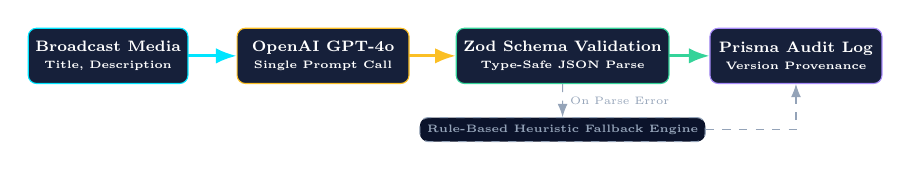
\begin{tikzpicture}[scale=0.78, every node/.style={transform shape, align=center}]
        \node[draw=omniCyan, fill=omniCard, rounded corners=3pt, font=\scriptsize\bfseries, text=white, minimum width=26mm, minimum height=9mm] (in) at (0,0) {Broadcast Media\\{\tiny Title, Description}};
        \node[draw=omniAmber, fill=omniCard, rounded corners=3pt, font=\scriptsize\bfseries, text=white, minimum width=28mm, minimum height=9mm] (llm) at (3.5,0) {OpenAI GPT-4o\\{\tiny Single Prompt Call}};
        \node[draw=omniGreen, fill=omniCard, rounded corners=3pt, font=\scriptsize\bfseries, text=white, minimum width=30mm, minimum height=9mm] (zod) at (7.4,0) {Zod Schema Validation\\{\tiny Type-Safe JSON Parse}};
        \node[draw=omniPurple, fill=omniCard, rounded corners=3pt, font=\scriptsize\bfseries, text=white, minimum width=28mm, minimum height=9mm] (audit) at (11.2,0) {Prisma Audit Log\\{\tiny Version Provenance}};

        \draw[-{Latex}, omniCyan, line width=1pt] (in) -- (llm);
        \draw[-{Latex}, omniAmber, line width=1pt] (llm) -- (zod);
        \draw[-{Latex}, omniGreen, line width=1pt] (zod) -- (audit);

        \node[draw=omniSlate, dashed, fill=omniDark, rounded corners=3pt, font=\tiny\bfseries, text=omniSlate] (fall) at (7.4,-1.2) {Rule-Based Heuristic Fallback Engine};
        \draw[-{Latex}, omniSlate, dashed] (zod) -- node[right, font=\tiny]{On Parse Error} (fall);
        \draw[-{Latex}, omniSlate, dashed] (fall) -| (audit);
      \end{tikzpicture}
    \end{column}
  \end{columns}
  \vspace{1mm}
  \begin{columns}[t]
    \begin{column}{0.48\textwidth}
      \card{\linewidth}{omniGreen}{STRICT SCHEMA ENFORCEMENT}{
        \begin{itemize}
          \setlength\itemsep{1mm}
          \item Validates tags, target demographics, age ratings (G, PG, PG-13, R).
          \item Generates 3 catchy promotional headlines and EPG summaries.
        \end{itemize}
      }
    \end{column}
    \begin{column}{0.48\textwidth}
      \card{\linewidth}{omniPurple}{PRODUCTION RELIABILITY \& PROVENANCE}{
        \begin{itemize}
          \setlength\itemsep{1mm}
          \item Zero downtime: In case of API quota exhaustion, heuristic fallback engages.
          \item Full version history recorded: Every curation run tracks previous vs new tags.
        \end{itemize}
      }
    \end{column}
  \end{columns}
\end{frame}

% ============================================================
% SLIDE 8: gRPC Microservices & Realtime Streaming Ingest
% ============================================================
\begin{frame}{Microservices \& Streaming Ingest}{High-Speed Audit Logging \& MediaMTX WebRTC Pipeline}
  \begin{columns}[t]
    \begin{column}{0.48\textwidth}
      \card{\linewidth}{omniPurple}{gRPC AUDIT-LOGGER MICROSERVICE}{
        \begin{itemize}
          \setlength\itemsep{1.2mm}
          \item \textbf{Technology:} NestJS Microservice + Protocol Buffers v3 (\texttt{audit.proto}).
          \item \textbf{Transport:} High-performance binary HTTP/2 transport over port \texttt{50051}.
          \item \textbf{Zero Main-Thread Blocking:} Asynchronously logs critical events:
            \begin{itemize}
              \item Program schedule additions and cancellations.
              \item Admin user role escalations.
              \item AI curation executions and manual overrides.
            \end{itemize}
          \item \textbf{Cloud Deployment:} Render Cloud Container.
        \end{itemize}
      }
    \end{column}

    \begin{column}{0.48\textwidth}
      \card{\linewidth}{omniAmber}{MEDIAMTX REALTIME STREAMING NODE}{
        \begin{itemize}
          \setlength\itemsep{1.2mm}
          \item \textbf{Ingest Protocol (WHIP):} WebRTC HTTP Ingestion Protocol allows web studio browsers to broadcast directly from webcams.
          \item \textbf{Distribution Protocol (WHEP \& HLS):} Sub-500ms ultra-low latency WebRTC streaming with HLS fallback for constrained networks.
          \item \textbf{Interactive WebSocket Gateway:}
            \begin{itemize}
              \item Real-time viewer counter (CCU calculation).
              \item Floating emoji reactions broadcasting.
              \item Live chat room pub/sub with message moderation.
            \end{itemize}
        \end{itemize}
      }
    \end{column}
  \end{columns}
\end{frame}

% ============================================================
% SLIDE 9: Web Portal Architecture (Next.js 15 App Router)
% ============================================================
\begin{frame}{Web Portal Architecture}{Next.js 15 App Router, React 19 \& Cinema Dark UI}
  \begin{columns}[t]
    \begin{column}{0.48\textwidth}
      \card{\linewidth}{omniBlue}{MODERN NEXT.JS 15 APP ROUTER}{
        \begin{itemize}
          \setlength\itemsep{1.2mm}
          \item \textbf{33 Application Routes:} Clean division into public portal, authenticated studio, and admin console.
          \item \textbf{Server Component Performance:} Zero client bundle weight for static metadata, EPG grids, and SEO indexing.
          \item \textbf{Optimized Client Hydration:} Dynamic interactive widgets only where necessary (OmniVideoPlayer, LiveChat).
        \end{itemize}
      }
    \end{column}

    \begin{column}{0.48\textwidth}
      \card{\linewidth}{omniCyan}{KEY USER FACING MODULES}{
        \begin{itemize}
          \setlength\itemsep{1.2mm}
          \item \textbf{Broadcast Studio (\texttt{/studio}):} Ingests webcam stream, manages active live events, and edits program schedules.
          \item \textbf{Live Curator Workspace (\texttt{/studio/curator}):} Interactive AI inspection, tagging overrides, and history comparison.
          \item \textbf{Admin Telemetry (\texttt{/admin}):} Real-time spline curves monitoring CCU, CDN bandwidth, and audit trails.
        \end{itemize}
      }
    \end{column}
  \end{columns}
\end{frame}

% ============================================================
% SLIDE 10: PRN232 Verification & Quality Assurance
% ============================================================
\begin{frame}{PRN232 Verification \& Testing}{391 Automated Tests Across Back-End \& Web Portal}
  \begin{columns}[t]
    \begin{column}{0.48\textwidth}
      \card{\linewidth}{omniGreen}{BACK-END AUTOMATED TEST SUITE (163 TESTS)}{
        \begin{itemize}
          \setlength\itemsep{1.2mm}
          \item \textbf{Framework:} Node.js native test runner (\texttt{node:test}).
          \item \textbf{Core Coverage:}
            \begin{itemize}
              \item Airtime collision interval edge cases (14 tests).
              \item Seeded EPG generator determinism (12 tests).
              \item JWT authentication \& RBAC guard enforcement (38 tests).
              \item AI Curator fallback and validation error handling (19 tests).
            \end{itemize}
          \item \textbf{Status:} 163/163 PASS (100\% Success Rate).
        \end{itemize}
      }
    \end{column}

    \begin{column}{0.48\textwidth}
      \card{\linewidth}{omniBlue}{WEB PORTAL \& E2E TESTING (228+8 TESTS)}{
        \begin{itemize}
          \setlength\itemsep{1.2mm}
          \item \textbf{Component Unit Testing:} 228 Vitest tests validating UI components, forms, and client API states.
          \item \textbf{End-to-End Browser Testing:} 8 comprehensive Playwright E2E scenarios with verified screenshots:
            \begin{itemize}
              \item Authentication flow (Login, Register, Invalid creds).
              \item Channel catalog browsing \& category filtering.
              \item EPG 24-hour timeline rendering and live viewing.
            \end{itemize}
          \item \textbf{Status:} 100\% Verified in CI/CD Pipeline.
        \end{itemize}
      }
    \end{column}
  \end{columns}
\end{frame}

% ============================================================
% PART 2 DIVIDER
% ============================================================
\section{PRM393 Mobile Client}
{
\setbeamertemplate{headline}{}
\begin{frame}[plain]
  \begin{tikzpicture}[remember picture, overlay]
    \fill[omniDeep] (current page.north west) rectangle (current page.south east);
    \fill[omniPurple!10] ($(current page.north west) + (0,-15mm)$) rectangle ($(current page.south east) + (0,15mm)$);
  \end{tikzpicture}
  \begin{center}
    \vspace{10mm}
    {\scriptsize\bfseries\color{omniCyan}MODULE 2 OF 2}\\[3mm]
    {\Huge\bfseries\color{white}PART 2: PRM393}\\[3mm]
    {\Large\bfseries\color{omniPurple}Mobile Applications Development}\\[4mm]
    {\color{omniBorder}\rule{0.5\linewidth}{1pt}}\\[4mm]
    {\footnotesize\color{omniSlate}Flutter 3.x $\bullet$ Dart $\bullet$ Clean Architecture $\bullet$ BLoC Pattern $\bullet$ Offline SQLite $\bullet$ OmniPlayer}
  \end{center}
\end{frame}
}

% ============================================================
% SLIDE 11: Mobile Architecture & Clean Architecture Pattern
% ============================================================
\begin{frame}{Mobile Architecture \& Patterns}{Four-Tier Clean Architecture with 12 BLoC State Machines}
  \begin{columns}[t]
    \begin{column}{0.48\textwidth}
      \card{\linewidth}{omniPurple}{FOUR-TIER CLEAN ARCHITECTURE}{
        \begin{itemize}
          \setlength\itemsep{1.2mm}
          \item \textbf{1. Core Layer:} Dependency Injection via \texttt{get\_it}, HTTP Dio client with JWT interceptors, Theme constants, Network info.
          \item \textbf{2. Data Layer:} Repositories, DTO models with JSON serialization, local SQLite \texttt{DatabaseHelper}.
          \item \textbf{3. Logic Layer:} 12 BLoC and Cubit modules managing asynchronous reactive state streams.
          \item \textbf{4. Presentation Layer:} 31 screens, modular UI components, OmniPlayer, GoRouter navigation.
        \end{itemize}
      }
    \end{column}

    \begin{column}{0.48\textwidth}
      \card{\linewidth}{omniCyan}{REACTIVE BLOC STATE MANAGEMENT}{
        \begin{itemize}
          \setlength\itemsep{1.2mm}
          \item \textbf{Predictable State Machine:} Strict separation between Events, Business Logic, and Immutable UI States.
          \item \textbf{12 Specialized BLoCs:}
            \begin{itemize}
              \item \texttt{AuthBloc}: JWT session, biometric token storage.
              \item \texttt{ChannelsBloc} \& \texttt{EpgBloc}: Catalog \& grid state.
              \item \texttt{WatchlistBloc}: Offline bookmarking \& sync.
              \item \texttt{OmniPlayerCubit}: Streaming playback control.
              \item \texttt{LiveChatCubit}: WebSocket messaging \& donation.
            \end{itemize}
          \item \textbf{Zero Memory Leaks:} Proper stream lifecycle closure.
        \end{itemize}
      }
    \end{column}
  \end{columns}
\end{frame}

% ============================================================
% SLIDE 12: Mobile Contribution 1 - Offline-First SQLite Engine
% ============================================================
\begin{frame}{Mobile Contribution 1: Offline-First SQLite Engine}{Local Caching with Asynchronous Mutation Replay Queue}
  \begin{columns}[t]
    \begin{column}{0.52\textwidth}
      \card{\linewidth}{omniGreen}{DUAL-LAYER DATA SYNCHRONIZATION}{
        \begin{itemize}
          \setlength\itemsep{1.2mm}
          \item \textbf{Offline Availability:} Users can browse cached channels, read EPG schedules, and check program details with zero connectivity.
          \item \textbf{Local SQLite Schema:}
            \begin{itemize}
              \item \texttt{cached\_channels}: Fast cold-start catalog display.
              \item \texttt{cached\_programs}: 24-hour schedule storage.
              \item \texttt{watchlist}: Saved user favorites.
              \item \texttt{offline\_mutations}: Pending queued mutations.
            \end{itemize}
          \item \textbf{Advance Local Alarms:} Exact 15-minute advance broadcast notification alerts scheduled locally via OS alarm manager.
        \end{itemize}
      }
    \end{column}

    \begin{column}{0.44\textwidth}
      \card{\linewidth}{omniTeal}{MUTATION REPLAY QUEUE}{
        \begin{center}
        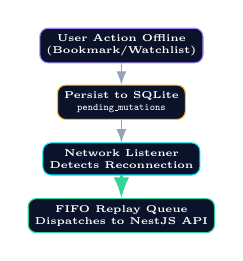
\begin{tikzpicture}[scale=0.72, every node/.style={transform shape, align=center}]
          \node[draw=omniPurple, fill=omniDark, rounded corners=3pt, font=\tiny\bfseries, text=white] (act) at (0,2.1) {User Action Offline\\(Bookmark/Watchlist)};
          \node[draw=omniAmber, fill=omniDark, rounded corners=3pt, font=\tiny\bfseries, text=white] (sql) at (0,1.1) {Persist to SQLite\\\texttt{pending\_mutations}};
          \node[draw=omniCyan, fill=omniDark, rounded corners=3pt, font=\tiny\bfseries, text=white] (net) at (0,0.1) {Network Listener\\Detects Reconnection};
          \node[draw=omniGreen, fill=omniDark, rounded corners=3pt, font=\tiny\bfseries, text=white] (sync) at (0,-0.9) {FIFO Replay Queue\\Dispatches to NestJS API};

          \draw[-{Latex}, omniSlate] (act) -- (sql);
          \draw[-{Latex}, omniSlate] (sql) -- (net);
          \draw[-{Latex}, omniGreen, line width=1pt] (net) -- (sync);
        \end{tikzpicture}
        \end{center}
      }
    \end{column}
  \end{columns}
\end{frame}

% ============================================================
% SLIDE 13: Mobile Contribution 2 - OmniPlayer & Dynamic LAN Discovery
% ============================================================
\begin{frame}{Mobile Contribution 2: OmniPlayer Streaming}{Multi-Engine WebRTC/HLS with Dynamic In-App LAN Discovery}
  \begin{columns}[t]
    \begin{column}{0.48\textwidth}
      \card{\linewidth}{omniAmber}{MULTI-ENGINE OMNIPLAYER}{
        \begin{itemize}
          \setlength\itemsep{1.2mm}
          \item \textbf{Ultra-Low Latency WebRTC:} Directly connects to MediaMTX WHEP endpoint for real-time live video (<500ms).
          \item \textbf{Adaptive HLS Fallback:} Seamlessly falls back to HLS \texttt{.m3u8} stream if WebRTC signaling fails.
          \item \textbf{Mobile Controls:} Aspect ratio toggling (16:9, fit, cover), Picture-in-Picture (PiP), and hardware-accelerated rendering.
        \end{itemize}
      }
    \end{column}

    \begin{column}{0.48\textwidth}
      \card{\linewidth}{omniCyan}{DYNAMIC LAN HOST DISCOVERY}{
        \begin{itemize}
          \setlength\itemsep{1.2mm}
          \item \textbf{The Mobile Testing Challenge:} Android physical devices cannot reach \texttt{localhost:8888} of the development machine.
          \item \textbf{Dynamic In-App Configuration:}
            \begin{itemize}
              \item Built-in host discovery sheet allows overriding MediaMTX host IP on-the-fly without rebuilding APK.
              \item Automatically resolves host IP for zero-fallback camera playback during live grading and testing.
            \end{itemize}
        \end{itemize}
      }
    \end{column}
  \end{columns}
\end{frame}

% ============================================================
% SLIDE 14: Mobile Contribution 3 - Interactive Real-Time Ecosystem
% ============================================================
\begin{frame}{Mobile Contribution 3: Interactive Streaming}{Live Chat, Floating Particle Reactions \& Virtual Donations}
  \begin{columns}[t]
    \begin{column}{0.32\textwidth}
      \card{\linewidth}{omniCyan}{REAL-TIME LIVE CHAT}{
        \begin{itemize}
          \setlength\itemsep{1mm}
          \item Socket.IO client connected to \texttt{/live} gateway.
          \item Fast optimistic message rendering.
          \item User avatar, role badges (VIP, Mod, Admin).
          \item System announcement broadcast banners.
        \end{itemize}
      }
    \end{column}

    \begin{column}{0.32\textwidth}
      \card{\linewidth}{omniPurple}{FLOATING REACTIONS}{
        \begin{itemize}
          \setlength\itemsep{1mm}
          \item GPU-accelerated canvas particle physics.
          \item Tap reaction button produces floating hearts, fires, claps.
          \item Real-time broadcast sync across all connected viewers.
        \end{itemize}
      }
    \end{column}

    \begin{column}{0.32\textwidth}
      \card{\linewidth}{omniAmber}{SANDBOX LIVE DONATIONS}{
        \begin{itemize}
          \setlength\itemsep{1mm}
          \item 6 Virtual Gift Tiers (Coffee, Mic, Camera, Trophy, Star, Crown).
          \item Mock payment modal with instant celebratory confetti.
          \item 100\% risk-free educational sandbox gateway.
        \end{itemize}
      }
    \end{column}
  \end{columns}
\end{frame}

% ============================================================
% SLIDE 15: Mobile Navigation, UI/UX & PRM393 Testing
% ============================================================
\begin{frame}{Navigation \& Verification}{GoRouter 31 Screens \& 91 Automated Tests (100\% Pass)}
  \begin{columns}[t]
    \begin{column}{0.48\textwidth}
      \card{\linewidth}{omniBlue}{GOROUTER DECLARATIVE ROUTING}{
        \begin{itemize}
          \setlength\itemsep{1.2mm}
          \item \textbf{31 Distinct Screens:} Spanning Auth, Catalog, EPG, Player, Creator Studio, Watchlist, Settings.
          \item \textbf{Auth Guard Redirects:} Automatic redirection if JWT token expires or required roles are missing.
          \item \textbf{Cinema Dark Aesthetic:} High-contrast UI optimized for OLED screens, haptic feedback on touch gestures.
        \end{itemize}
      }
    \end{column}

    \begin{column}{0.48\textwidth}
      \card{\linewidth}{omniGreen}{91 AUTOMATED TESTS (100\% PASS)}{
        \begin{itemize}
          \setlength\itemsep{1.2mm}
          \item \textbf{Unit Tests (56 tests):} BLoC state transition testing (\texttt{bloc\_test}), SQLite repository operations, DTO serialization.
          \item \textbf{Widget Tests (35 tests):} UI component rendering, button interactions, mock network failure handlers.
          \item \textbf{CI/CD Integration:} Tested automatically on every git commit via GitHub Actions.
        \end{itemize}
      }
    \end{column}
  \end{columns}
\end{frame}

% ============================================================
% PART 3: SYNERGY & DEPLOYMENT
% ============================================================
\section{Synergy \& Deployment}
\begin{frame}{Cross-Platform Synergy Matrix}{Side-by-Side Comparison: PRN232 Back-End vs PRM393 Mobile}
  \begin{center}
  \footnotesize
  \renewcommand{\arraystretch}{1.2}
  \begin{tabularx}{0.95\linewidth}{lXX}
    \toprule
    \textbf{Dimension} & \textbf{\color{omniCyan}PRN232 (Back-End \& Web)} & \textbf{\color{omniPurple}PRM393 (Mobile App)} \\
    \midrule
    \textbf{Core Framework} & NestJS 10 + Next.js 15 App Router & Flutter 3.x + Dart 3 \\
    \textbf{Architecture} & Layered Clean Modules + gRPC & 4-Tier Clean Architecture + BLoC \\
    \textbf{Database / Cache} & Supabase PostgreSQL (21 models) & SQLite Local (\texttt{sqflite}) + SharedPrefs \\
    \textbf{Streaming Role} & Ingest (WHIP), Signaling, EPG & Player (WHEP/HLS), Floating UI \\
    \textbf{Realtime Engine} & Socket.IO Gateway Server (\texttt{/live}) & Socket.IO Client + Particle Canvas \\
    \textbf{Code Volume} & \textbf{79,568 Physical LOC} & \textbf{53,922 Physical LOC} \\
    \textbf{Automated Tests} & \textbf{391 Tests} (163 API + 228 Web) & \textbf{91 Tests} (Unit + Widgets) \\
    \textbf{Verification Rate} & \textbf{100\% PASS} & \textbf{100\% PASS} \\
    \bottomrule
  \end{tabularx}
  \end{center}
  \vspace*{-1mm}
  \begin{center}
    \scriptsize\color{omniGreen}\textbf{TOTAL SYSTEM SCALE: 142,897 Lines of Code $\bullet$ 482 Automated Tests $\bullet$ 100\% Pass}
  \end{center}
\end{frame}

% ============================================================
% SLIDE 17: Live Production Deployment & Demo Accounts
% ============================================================
\begin{frame}{Live Deployment \& Evaluation}{Production Cloud Infrastructure \& Pre-Seeded Test Credentials}
  \begin{columns}[t]
    \begin{column}{0.52\textwidth}
      \card{\linewidth}{omniBlue}{LIVE PRODUCTION ENDPOINTS}{
        \begin{itemize}
          \setlength\itemsep{1.2mm}
          \item \textbf{Web Portal (Vercel Live):}\\
            \href{https://omnicast-fe.vercel.app}{\color{omniCyan}\texttt{https://omnicast-fe.vercel.app}}
          \item \textbf{Core API Swagger Documentation:}\\
            \href{https://omnicast-api.vercel.app/swagger}{\color{omniCyan}\texttt{https://omnicast-api.vercel.app/swagger}}
          \item \textbf{Mobile APK Release (v1.2.0):}\\
            \texttt{github.com/TomOutfit/.../releases/tag/v1.2.0}
          \item \textbf{Official GitHub Repository:}\\
            \texttt{github.com/TomOutfit/OmniCast\_PRN232-PRM393...}
        \end{itemize}
      }
    \end{column}

    \begin{column}{0.44\textwidth}
      \card{\linewidth}{omniGreen}{PRE-CONFIGURED EVALUATION ACCOUNTS}{
        \textbf{Password for all test accounts:} \texttt{Admin123!}
        \vspace{2mm}
        \begin{itemize}
          \setlength\itemsep{1.5mm}
          \item \textbf{Admin Account (Full RBAC):}\\
            \texttt{admin@omnicast.tv}
          \item \textbf{Staff Account (Studio Broadcaster):}\\
            \texttt{staff@omnicast.tv}
          \item \textbf{Viewer Account (Consumer):}\\
            \texttt{viewer1@omnicast.tv}
        \end{itemize}
      }
    \end{column}
  \end{columns}
\end{frame}

% ============================================================
% SLIDE 18: Project Milestones & Lessons Learned
% ============================================================
\begin{frame}{Project Milestones \& Lessons Learned}{Engineering Takeaways from Joint Capstone Implementation}
  \begin{columns}[t]
    \begin{column}{0.48\textwidth}
      \card{\linewidth}{omniCyan}{KEY TECHNICAL ACHIEVEMENTS}{
        \begin{itemize}
          \setlength\itemsep{1.2mm}
          \item Successfully bridged complex broadcast engineering with cloud-native web and native mobile clients.
          \item Eliminated airtime overlap risks through atomic SQL interval calculation.
          \item Solved the 24/7 dead air dilemma using deterministic seeded pseudo-random filling.
          \item Provided seamless offline resilience for mobile users through SQLite mutation queuing.
        \end{itemize}
      }
    \end{column}

    \begin{column}{0.48\textwidth}
      \card{\linewidth}{omniAmber}{LESSONS LEARNED \& FUTURE EXTENSIONS}{
        \begin{itemize}
          \setlength\itemsep{1.2mm}
          \item \textbf{gRPC Efficiency:} Binary proto serialization drastically reduces latency compared to conventional REST.
          \item \textbf{BLoC Event Isolation:} Strict event streams prevent UI stuttering during heavy network calls.
          \item \textbf{Future Work:} Distributed MediaMTX clustering across edge nodes, AI auto-dubbing, and adaptive multi-bitrate transcoding.
        \end{itemize}
      }
    \end{column}
  \end{columns}
\end{frame}

% ============================================================
% SLIDE 19: Conclusion & Q&A
% ============================================================
\section{Conclusion}
{
\setbeamertemplate{headline}{}
\setbeamertemplate{footline}{}
\begin{frame}[plain]
  \begin{tikzpicture}[remember picture, overlay]
    \fill[omniDeep] (current page.north west) rectangle (current page.south east);
    \draw[omniCyan!30, line width=0.8pt, dashed] ($(current page.north west) + (10mm,-10mm)$) rectangle ($(current page.south east) + (-10mm,10mm)$);
    \draw[omniBorder, line width=1.2pt] ($(current page.north west) + (12mm,-12mm)$) rectangle ($(current page.south east) + (-12mm,12mm)$);
  \end{tikzpicture}
  \begin{center}
    \vspace{8mm}
    {\Huge\bfseries\color{white}Thank You for Your Attention!}\\[3mm]
    {\large\bfseries\color{omniCyan}OmniCast: Enterprise Media \& Broadcast Intelligence Network}\\[4mm]
    {\color{omniBorder}\rule{0.6\linewidth}{1pt}}\\[5mm]

    {\normalsize\bfseries\color{white}We are ready for Live Demonstration \& Committee Q\&A}\\[6mm]

    
\begin{tikzpicture}
      \node[draw=omniCyan, fill=omniCard, rounded corners=3pt, text=white, font=\scriptsize] (w1) at (-4,0) {
        \textbf{Web:} \texttt{omnicast-fe.vercel.app}
      };
      \node[draw=omniPurple, fill=omniCard, rounded corners=3pt, text=white, font=\scriptsize] (w2) at (0,0) {
        \textbf{API:} \texttt{omnicast-api.vercel.app/swagger}
      };
      \node[draw=omniGreen, fill=omniCard, rounded corners=3pt, text=white, font=\scriptsize] (w3) at (4.5,0) {
        \textbf{GitHub:} \texttt{github.com/TomOutfit/OmniCast}
      };
    \end{tikzpicture}
    \vspace{5mm}

    {\scriptsize\color{omniSlate}Department of Software Engineering $\bullet$ FPT University $\bullet$ Fall 2026}
  \end{center}
\end{frame}
}

\end{document}
